The equation of circle can be expressed as
\begin{align}
    \vec{x}^T\vec{x}-2\vec{c}^T\vec{x}+f = 0
\end{align}
$\vec{c}$ is the centre  and substituting the points in the equation of circle we get
\begin{align}
2\myvec{2a&0}\vec{c}-f=4a^2\\
2\myvec{0&2b}\vec{c}-f=4b^2\\
2\myvec{a+b&a+b}\vec{c}-f=2\brak{a+b}^2
\end{align}
which can be expressed in matrix form
\begin{align}
\myvec{4a&0&-1\\0&4b&-1\\2\brak{a+b}&2\brak{a+b}&-1}\myvec{\vec{c}\\f} = \myvec{4a^2\\4b^2\\2\brak{a+b}^2}
\end{align}
Row reducing the augmented matrix
\begin{align}
\myvec{4a&0&-1&4a^2\\0&4b&-1&4b^2\\2\brak{a+b}&2\brak{a+b}&-1&2\brak{a+b}^2}\\
\xleftrightarrow[R_3\leftarrow R_3-2\brak{a+b}R_1]{R_1\leftarrow \frac{R_1}{4 a}}
\myvec{1 & 0 & - \frac{1}{4 a} & a \\ 0 & 4 b & -1 & 4 b^{2} \\ 0 & 2 \brak{a + b}& \frac{-a + b}{2 a} & 2b\brak{a + b}}\\
\xleftrightarrow[R_2\leftarrow \frac{R_2}{4 b}]{R_3\leftarrow R_3-2\brak{a + b}R_2}
\myvec{1 & 0 & - \frac{1}{4 a} & a \\ 0 & 1 & - \frac{1}{4 b} & b \\ 0 & 0 & \frac{a}{2 b} + \frac{b}{2 a} & 0}\\
\xleftrightarrow[]{R_3\leftarrow \frac{R_3}{\frac{a}{2b} + \frac{b}{2a}}}
\myvec{1 & 0 & - \frac{1}{4 a} & a \\ 0 & 1 & - \frac{1}{4 b} & b \\ 0 & 0 & 1 & 0}\\
\xleftrightarrow[R_1\leftarrow R_1-\brak{-\frac{1}{4 a}}R_3]{R_2\leftarrow R_2-\brak{-\frac{1}{4 b}}R_3}
\myvec{1 & 0 & 0 & a \\ 0 & 1 & 0 & b \\ 0 & 0 & 1 & 0}
\end{align}
\begin{align}
    \vec{c} = \myvec{a\\b}\\
    f = 0\\
    r=\sqrt{\norm{\vec{c}}^2-f} = \sqrt{\brak{a^2+b^2}}
\end{align}
The required equation of circle is 
\begin{align}
\vec{x}^T\vec{x}-2\myvec{a&b}\vec{x} = 0
\end{align}
\begin{figure}[!ht]
\centering
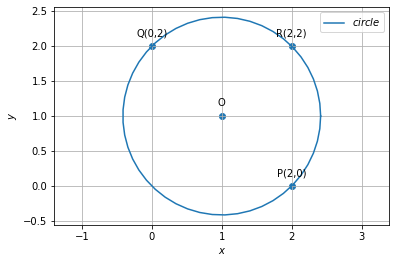
\includegraphics[width=\columnwidth]{./solutions/4/1/4/5.png}
\caption{Circle passing through point P and Q and R}
\label{eq:solutions/4/1/4/Fig:5}
\end{figure}

